\documentclass{article}

\usepackage{graphicx}
\usepackage{tikz}
\usepackage{tikzsymbols}
\usetikzlibrary{calc,patterns,shapes.geometric}
\pagestyle{empty}
\usepackage[margin=0pt]{geometry}
\geometry{papersize={14in,12in}}

\def\centerarc[#1](#2)(#3:#4:#5){\draw[#1] ($(#2)+({#5*cos(#3)},{#5*sin(#3)})$) arc (#3:#4:#5);}

\begin{document}
	\begin{figure}
		\centering
		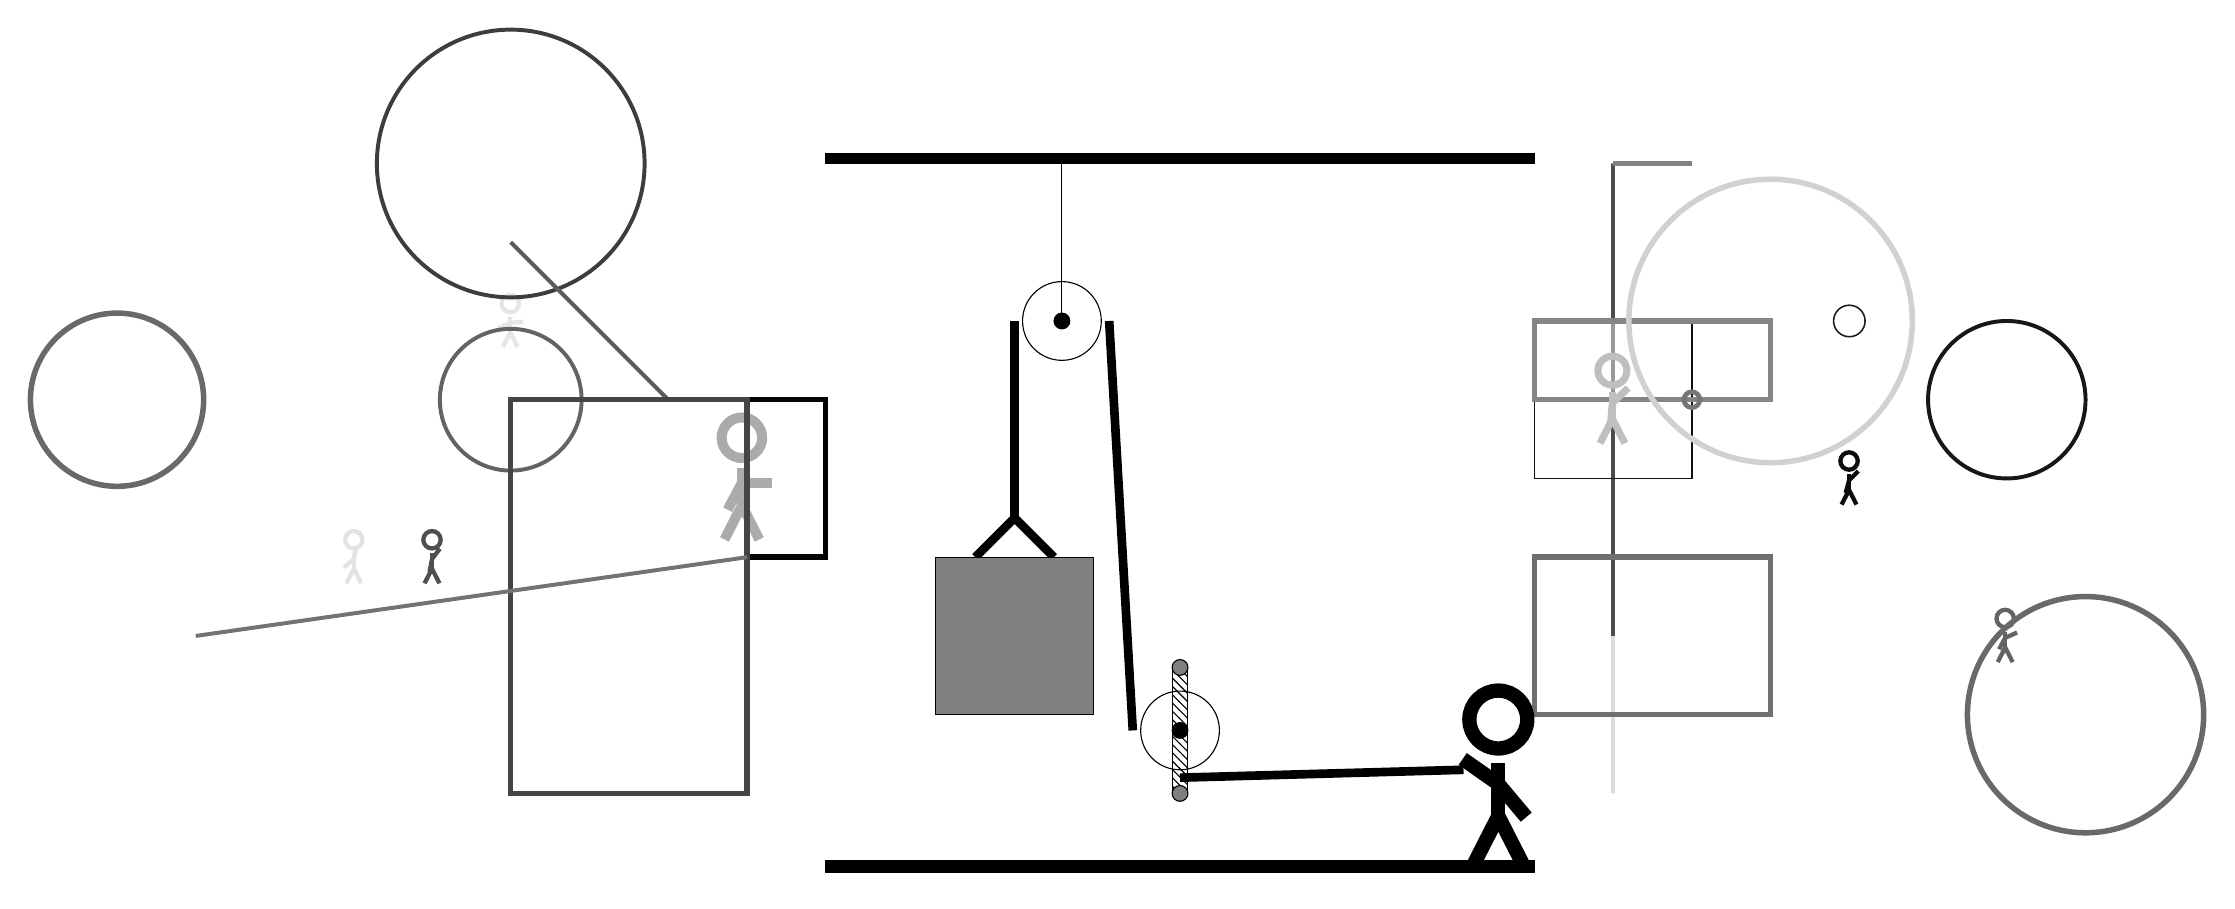
\begin{tikzpicture}
			%%%%% START %%%%%
			
			\draw[fill=black] (-2, 9) rectangle (7, 9.125);
			
			\draw (1, 7) circle (0.5);
			\draw[fill=black] (1, 7) circle (0.1);
			\draw (1, 9) -- (1, 7);
			
			\node[line width=0.3mm, color=black!10] at (-6, 7) {\Strichmaxerl[3][24][5]};
			
			\draw [line width=0.5mm, color=black!61](-6, 6) circle (0.9);
			\draw [line width=0.5mm, color=black!76](-6, 9) circle (1.7);
			\node[line width=0.5mm, color=black!61] at (13, 3) {\Strichmaxerl[3][62][24]};
			\draw[line width=0.6mm, color=black!14] (8, 1) rectangle (8, 3);
			\draw [line width=0.2mm, color=black!89](11, 7) circle (0.2);
			\node[line width=0.3mm, color=black!33] at (-3, 5) {\Strichmaxerl[7][62][0]};
			\draw[line width=0.5mm, color=black!64](-6, 8) -- (-4, 6);
			\draw [line width=0.5mm, color=black!91](13, 6) circle (1.0);
			\draw[line width=0.6mm, color=black!70] (8, 9) rectangle (8, 3);
			
			\draw[line width=0.7mm, color=black!99] (-2, 6) rectangle (-3, 4);
			\draw[line width=0.5mm, color=black!40] (7, 7) rectangle (8, 6);
			\draw[line width=0.2mm, color=black!94] (7, 7) rectangle (9, 5);
			
			\draw [line width=0.7mm, color=black!59](-11, 6) circle (1.1);
			\draw[line width=0.7mm, color=black!48] (7, 7) rectangle (10, 6);
			\draw [line width=0.7mm, color=black!18](10, 7) circle (1.8);
			
			\draw [line width=0.7mm, color=black!59](14, 2) circle (1.5);
			\node[line width=0.5mm, color=black!95] at (11, 5) {\Strichmaxerl[3][75][45]};
			\draw[line width=0.7mm, color=black!73] (-3, 1) rectangle (-6, 6);
			\draw [line width=0.6mm, color=black!54](9, 6) circle (0.1);
			\node[line width=0.4mm, color=black!11] at (-8, 4) {\Strichmaxerl[3][41][77]};
			
			\node[line width=0.4mm, color=black!25] at (8, 6) {\Strichmaxerl[5][85][43]};
			\draw[line width=0.7mm, color=black!56] (7, 4) rectangle (10, 2);
			\draw[line width=0.6mm, color=black!49] (9, 9) rectangle (8, 9);
			\node[line width=0.2mm, color=black!69] at (-7, 4) {\Strichmaxerl[3][79][53]};
			
			\draw[line width=0.5mm, color=black!55](-3, 4) -- (-10, 3);
			
			\draw[fill=white](2.5, 1.8) circle (0.5);
			\draw[fill=black] (2.5, 1.8) circle (0.1);
			\draw[pattern=north west lines, pattern color=black] (2.4, 2.6) rectangle (2.6, 1.0);
			\draw[fill=black!50] (2.5, 2.6) circle (0.1);
			\draw[fill=black!50] (2.5, 1.0) circle (0.1);
			
			\draw[line width=1.1mm] (-0.1, 4.0) -- (0.4, 4.5) -- (0.9, 4.0);
			\draw[fill=black!50] (-0.6, 4.0) rectangle (1.4, 2.0);
			
			\draw[line width=1.1mm] (0.4, 7) -- (0.4, 4.5);
			\centerarc[line width=1.1mm](1, 7)(0:180:0.6);
			\draw[line width=1.1mm](1.6, 7) -- (1.9, 1.8);
			\centerarc[line width=1.1mm](2.5, 1.8)(180:270:0.6);
			\draw[line width=1.1mm](2.5, 1.2) -- (6.1, 1.3);
			
			\node at (6.5, 1.2) {\Strichmaxerl[10][-35][-50]};
			
			\draw[fill=black] (-2, 0) rectangle (7, 0.15);
			
			%%%%% END %%%%%
		\end{tikzpicture}
	\end{figure}	
\end{document}